    \documentclass[12pt, a4paper]{report}
    \usepackage{/Users/vladbelousov/Desktop/Semestr_4-FP-NSU/Настройка/library}
    \usepackage[utf8]{inputenc} % Подключение поддержки UTF-8

\begin{document}

\chapter{Интерференция света. }

\section{Цель работы: }

Изучить интерференцию света на основе классических оптических схем реализации двухволновой интерференции:
интерферометр Майкельсона, схема Юнга, бипризма Френеля. На практике провести вычисления характеристик волны:
временная когерентность, контраст интерферирующих волн/полос.

\section{Теория: }

Cхема установки, позволяющей наблюдать интерференцию двух волн, с использованием интерферометра
Майкельсона, схемы Юнга и бипризмы Френеля. Установка содержит два модуля. Первый используется при работе с
интерферометром Майкельсона. Второй – при регистрации интерферограмм по схеме Юнга и с применением бипризмы
Френеля.

\begin{center}
    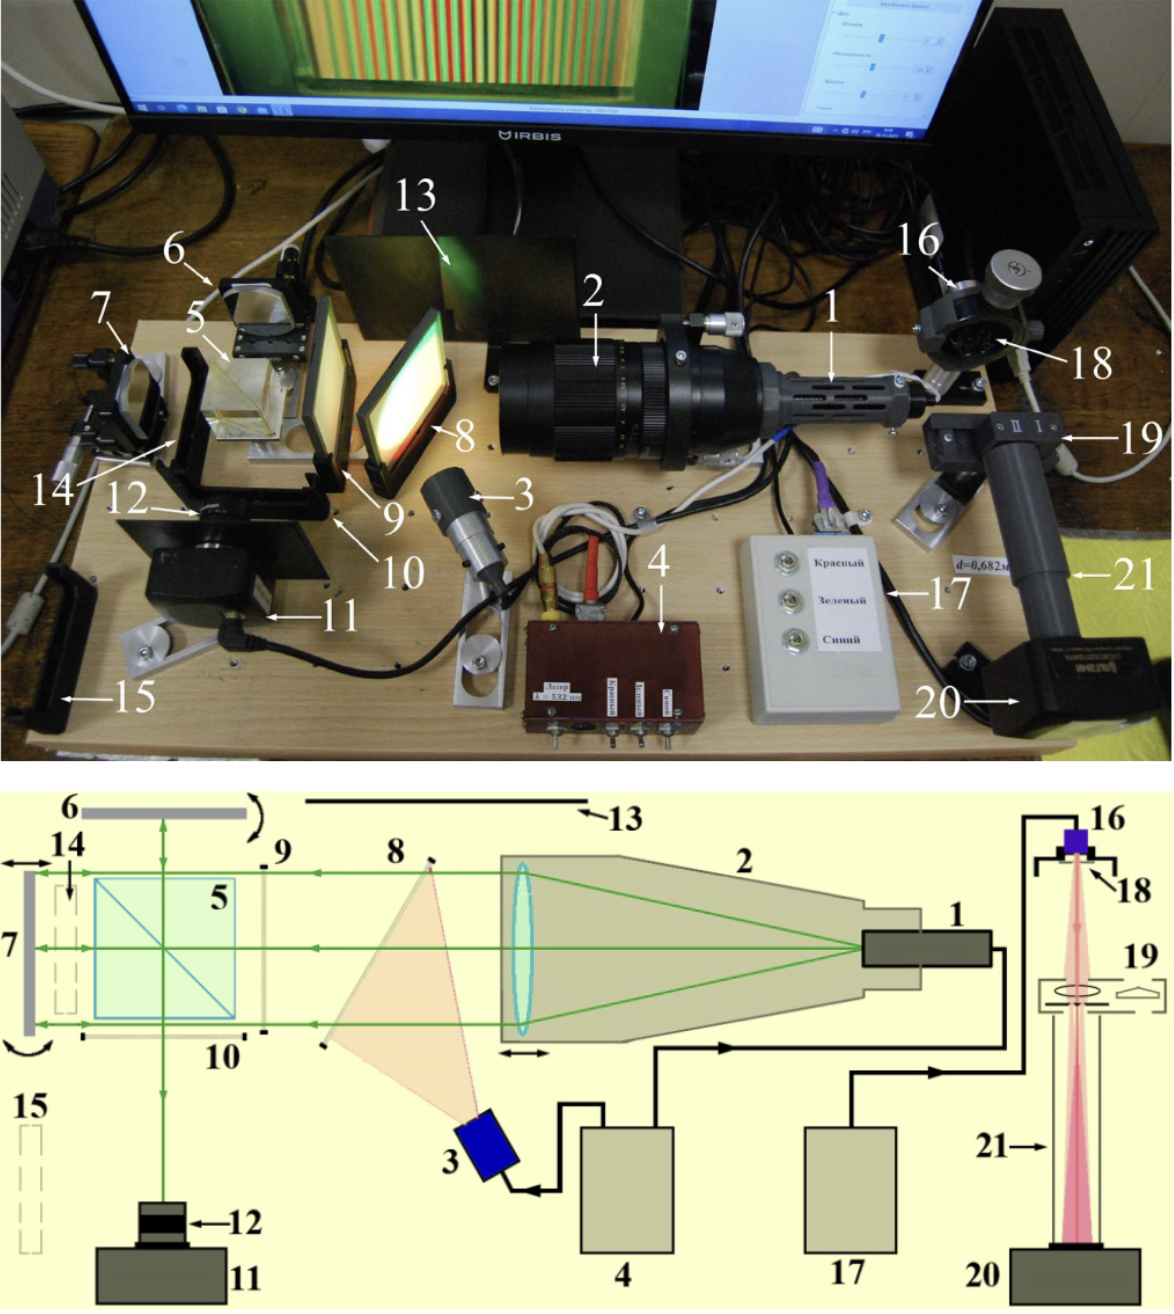
\includegraphics[width=0.65\textwidth]{image/1.png}
\end{center}

\newpage

\begin{flushleft}
    1. Модуль интерферометра Майкельсон:
\end{flushleft}

1) Лазер с длиной волны \( \lambda \approx\)   532 нм;

2) Объектив, который преобразует лазер в плоскопараллельный пучок, так же при помощи кольца резкости можно
расширить или уменьшить пучок;

3) Светодиод (красно, зеленый, синий);

4) Блок переключения при помощи которого управляются источники;

5) Светоделительный кубик, который делит излучение на две волны с 50-ти процентными коэффициентами
энергетического пропускания и отражения. Эти волны потом попадают на зеркала 6) и 7) снова отражаются и
идут опять на светоделительный кубик;

6) Зеркало;


7) Зеркало;

8) Светорассеивающий экран, который являются дополнительным источником освещения рассеивая назад ту
часть волны (50-ти процентов) которая проходит в сторону источника света;

9) Светорассеивающий экран тоже самое;

10) Экран, который ставят когда работают с коллимированным пучком от лазера;

11) Телекамера, на нее попадает другая половина энергии каждой волны выходящей из интерферометра. Именно
между этими волнами и наблюдается интерференция;

12) Кольцо резкости, на котором осуществляется регулировка резкости на объективе телекамеры;

13) Свето-поглощающий экран, нужен для техники безопастности;

14) Свето-поглощающий экран, может быть необходим для выполнения некоторых упражнений;

15) Светорассеивающий экран, может быть необходим для выполнения некоторых упражнений;

\begin{flushleft}
    2. Модуль для работы со схемой Юнга и бипризмой Френеля:
\end{flushleft}


16) Источник света, используется для схемы Юнга и биопризмы Френеля;

17) Блок переключения, нужен для управления 16);

18) Оптическая щель;

19) Оптика-механический бокс, включающий двухщелевую диафрагму и бипризму Френеля;

20) Телеэкран;

21) Светозащитный тубус;

\newpage 

\section{Задание 1: Определение длин волн светодиодных источников света}

Расстояние между двумя краями матрицы: 5,6 мм. N - это количество пиков, L - это расстояние между курсорами:

1. Зеленый лазер: N = 34, L = 2.76 мм, \( \lambda \) = 532.5 нм

2. Красный светодиод: N = 25, L = 2.43 мм, \( \lambda \) = 622 \( \pm \) 10 нм

3. Зеленый светодиод: N = 16, L = 1.32 мм, \( \lambda \) = 516 \( \pm \) 10 нм

4. Синий светодиод: N = 20, L = 1.49 мм, \( \lambda \) = 470 \( \pm \) 10 нм

Определим длину волны для каждого источника света по формуле: 

\[ h = \frac{\lambda}{ \Delta \alpha }  \] 

Где \( h \)  - это длина шага  наших интерференционных полос, которые определяются: \( \displaystyle h = \frac{L}{N}  \) 

Из реперной для заленого лазера: \( \displaystyle \Delta \alpha = \frac{\lambda_{\text{з.л} }}{h _{\text{з.л} }}  = \frac{\lambda _{\text{з.л} }N_{\text{з.л} }  }{L _{\text{з.л} }}  \) 

Итоговая формула для нахождения длин волн у светодиодов: 

\[ \lambda = \frac{L }{N} \frac{\lambda _{\text{з.л} }N_{\text{з.л} }  } {L _{\text{з.л} }}\] 

Расчетные данные: 

\[ \lambda_{Red} = 637.611 \text{ нм}  \] 

\[ \lambda_{Green} = 541.182 \text{ нм}  \] 

\[ \lambda_{Blue} = 488.704 \text{ нм}  \] 

\section{Задание 2: Определение длины когерентности излучения}

Количество интерференционных максимумов N в диапазоне изменения контраста в e раз: 

1. Зеленый лазер: N = 7

2. Красный светодиод: N = 10

3. Зеленый светодиод: N = 3

4. Синий светодиод: N = 5 

Через среднюю длину волны вычислим длину когерентности по формуле: 

\[ s_k = \lambda \cdot  N  \] 

Расчетные данные:

\[ s_{k_{Laser} }  = 4260 \text{нм}    \] 

\[ s_{k_{Red} }  = 6376.11 \text{нм}    \] 

\[ s_{k_{Green} }  = 1623.55 \text{нм}    \] 

\[ s_{k_{Blue} }  =  2443.52 \text{нм}    \] 

\section{Задание 3: Определение длины волны светодиодных источников
света и параметров схемы Юнга и схемы с бипризмой Френеля.}

Расстояние от двойной щели до камеры: \( S = 12.5 \text{ см } = 124  \) мм.

Расстояние между двумя пиками: 

1.  Зеленый светодиод: L = 0.49 мм

2. Красный светодиод: L = 0.57 мм

3. Синий светодиод: L = 0.43 мм

Как в задании два мы используем формул где из известной длины волны (в данном случа база это зеленый светодиод \( \lambda = 515 \text{ нм}  \)) получаем остальные: 

\[ \lambda = L \frac{\lambda _{\text{з} }  } {L _{\text{з} }}\] 

Расчетные данные:

\[ \lambda_{Red} = 599.663 \text{ нм}  \] 

\[ \lambda_{Blue} = 452.378\text{ нм}  \] 

Определим длину между щелями, воспользуемся формулой для угла: \( \displaystyle  \Delta \alpha  = \frac{d}{ S }  \), где d - это расстояние между щелями, а S - это расстояние от двойной щели до камеры.
\( \Delta \alpha  \) мы определим из формулы для длины волны: \( \displaystyle \Delta \alpha = \frac{\lambda}{h}   \). Итоговая формула для расстояния между щелями: 

\[ d = \frac{\lambda}{ h }  S = \frac{\lambda N }{L} S \] 

\[ d= 279 \text{ } 345 \text{ нм} = 0.27 \text{ мм} \] 

Для расчета длин при помощи биопризмы Френеля воспользуемся той-же формулой: 

\[ \lambda = \frac{L }{N} \frac{\lambda _{\text{з} }N_{\text{з} }  } {L _{\text{з} }}\] 

Расчетные данные: 

\[ \lambda_{Red} = 638.119 \text{ нм}  \] 

\[ \lambda_{Blue} = 459.537\text{ нм}  \] 

\section{Определение зависимости поперечной пространственной когерентности для схемы Юнга и схемы с бипризмой Френеля
от ширины щелевидного источника света.}

Явления рассматривались на примере синеного светоидода.

Описание явления для схемы Юнга: Самый первый пик мы увидели при 0.1 мм был светлый центр, после 0.1 мм у нас размывается картинка,нету явного "темного" или "светлого" центра, при 0.3 у нас проявляется пик в виде темного центра, то есть противофаза и так далее при прокручивании.

Описание явления для биопризмы Френеля: первый пик 0.7 мм светлый центр, 0.9 мм второй пик и тд.




\end{document}
